\documentclass[tikz,border=12pt]{standalone}
\usepackage[T1]{fontenc}
\usepackage{tgheros}
\usepackage{sfmath}
\usepackage{amsmath}
% % \usepackage{fontawesome5} (Removed for publication-grade academic typography) (Removed for publication-grade academic typography)
\usepackage{tikz}
\usetikzlibrary{arrows.meta,positioning,shapes.geometric,fit,backgrounds,calc}
\usepackage{xcolor}

\renewcommand{\familydefault}{\sfdefault}

% Harvard Crimson & ETH Zurich Academic Semantic Palette
\definecolor{harvardcrimson}{HTML}{A51C30}
\definecolor{ethdarkblue}{HTML}{1F407A}
\definecolor{ethblue}{HTML}{215CAF}
\definecolor{ethpetrol}{HTML}{007A87}
\definecolor{ethbronze}{HTML}{B87333}
\definecolor{ethpurple}{HTML}{5B4B8A}
\definecolor{ethslate}{HTML}{475569}
\definecolor{cardbg}{HTML}{F8FAFC}
\definecolor{cardborder}{HTML}{CBD5E1}
\definecolor{safeTeal}{HTML}{10B981}

\begin{document}
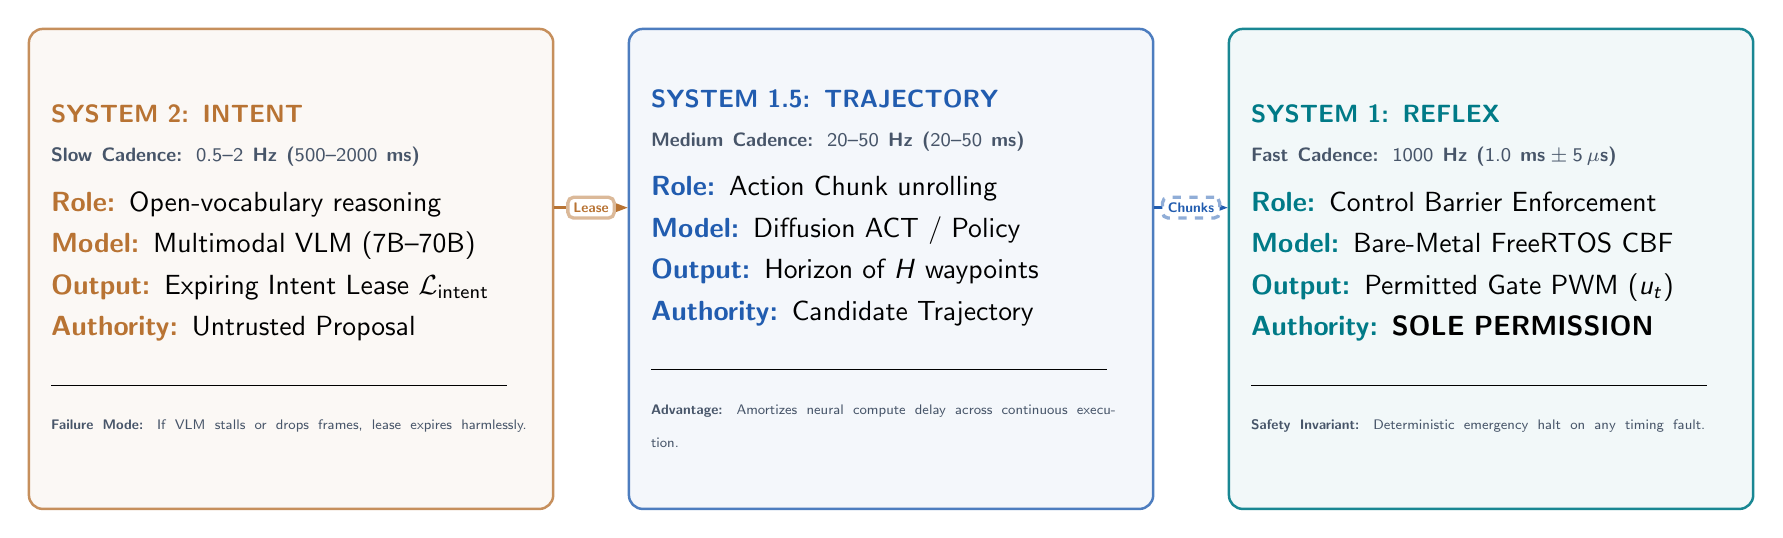
\begin{tikzpicture}[
  font=\sffamily,
  >=Stealth,
  cadencebox/.style={
    draw=cardborder,
    fill=cardbg,
    rounded corners=5pt,
    line width=0.9pt,
    text width=2.40in,
    minimum height=2.40in,
    inner sep=8pt,
    align=left,
    anchor=north west
  }
]

  % Top Title Banner
  % (Top title banner removed for academic publication standards)
% Column 1: System 2 (Semantic Intent)
  \node[cadencebox, draw=ethbronze!80, fill=ethbronze!5] (c1) at (0.20in, 0.00in) {
    {\small\bfseries\color{ethbronze} SYSTEM 2: INTENT}\\[2pt]
    {\scriptsize\bfseries\color{ethslate}Slow Cadence: $0.5\text{--}2\text{ Hz}$ ($500\text{--}2000\text{ ms}$)}\\[6pt]
    \textbf{\color{ethbronze}Role:} Open-vocabulary reasoning\\[3pt]
    \textbf{\color{ethbronze}Model:} Multimodal VLM ($7\text{B}\text{--}70\text{B}$)\\[3pt]
    \textbf{\color{ethbronze}Output:} Expiring Intent Lease $\mathcal{L}_{\text{intent}}$\\[3pt]
    \textbf{\color{ethbronze}Authority:} Untrusted Proposal\\[6pt]
    \rule{0.95\linewidth}{0.3pt}\\[4pt]
    {\tiny\color{ethslate}\textbf{Failure Mode:} If VLM stalls or drops frames, lease expires harmlessly.}
  };

  % Column 2: System 1.5 (Action Chunking)
  \node[cadencebox, draw=ethblue!80, fill=ethblue!5] (c2) at (3.20in, 0.00in) {
    {\small\bfseries\color{ethblue} SYSTEM 1.5: TRAJECTORY}\\[2pt]
    {\scriptsize\bfseries\color{ethslate}Medium Cadence: $20\text{--}50\text{ Hz}$ ($20\text{--}50\text{ ms}$)}\\[6pt]
    \textbf{\color{ethblue}Role:} Action Chunk unrolling\\[3pt]
    \textbf{\color{ethblue}Model:} Diffusion ACT / Policy\\[3pt]
    \textbf{\color{ethblue}Output:} Horizon of $H$ waypoints\\[3pt]
    \textbf{\color{ethblue}Authority:} Candidate Trajectory\\[6pt]
    \rule{0.95\linewidth}{0.3pt}\\[4pt]
    {\tiny\color{ethslate}\textbf{Advantage:} Amortizes neural compute delay across continuous execution.}
  };

  % Column 3: System 1 (Real-Time Reflex)
  \node[cadencebox, draw=ethpetrol!90, fill=ethpetrol!5] (c3) at (6.20in, 0.00in) {
    {\small\bfseries\color{ethpetrol} SYSTEM 1: REFLEX}\\[2pt]
    {\scriptsize\bfseries\color{ethslate}Fast Cadence: $1000\text{ Hz}$ ($1.0\text{ ms} \pm 5\,\mu\text{s}$)}\\[6pt]
    \textbf{\color{ethpetrol}Role:} Control Barrier Enforcement\\[3pt]
    \textbf{\color{ethpetrol}Model:} Bare-Metal FreeRTOS CBF\\[3pt]
    \textbf{\color{ethpetrol}Output:} Permitted Gate PWM ($u_t$)\\[3pt]
    \textbf{\color{ethpetrol}Authority:} \textbf{SOLE PERMISSION}\\[6pt]
    \rule{0.95\linewidth}{0.3pt}\\[4pt]
    {\tiny\color{ethslate}\textbf{Safety Invariant:} Deterministic emergency halt on any timing fault.}
  };

  % Flow arrows between cadences with clean non-colliding badge pills in the 0.60in gaps
  \draw[->, line width=1.2pt, ethbronze] ($(c1.north east) + (0, -0.90in)$) -- ($(c2.north west) + (0, -0.90in)$)
    node[midway, font=\sffamily\bfseries\tiny, fill=white, draw=ethbronze!50, rounded corners=2pt, inner sep=2pt, text=ethbronze] {Lease};

  \draw[->, line width=1.2pt, ethblue, dashed] ($(c2.north east) + (0, -0.90in)$) -- ($(c3.north west) + (0, -0.90in)$)
    node[midway, font=\sffamily\bfseries\tiny, fill=white, draw=ethblue!50, rounded corners=2pt, inner sep=2pt, text=ethblue] {Chunks};

\end{tikzpicture}
\end{document}
